\documentclass[resume]{subfiles}


\begin{document}
\section{Modulations}
\subsection{QAM}
\begin{center}
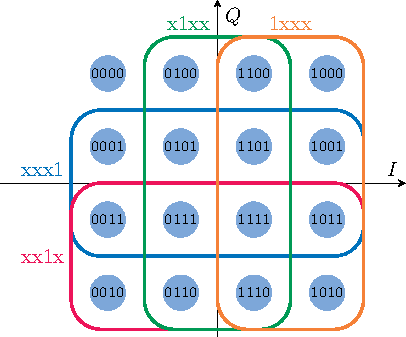
\includegraphics[scale=0.75]{drwg_5.pdf}
\end{center}
On utilise le codage de Grey. Si il y a une petite perturbation sur le signal, il y a un minimum de bits modifiées et donc la correction d'erreur pourra récupérer le message d'origine.



\end{document}